\section{Individual Work - Sven J. Steinert}

\subsection{GMAT Structure and Logic}
As the trajectory design and simulation inside GMAT have been one of the core elements, some sections are highlighted here from the final script \href{https://github.com/Sven-J-Steinert/MomenTUM/blob/main/GMAT/MomenTUM_finite.script}{\colorbox{codegray}{MomenTUM\_finite.script}}.
\\

\subsubsection{Finite Thruster Targeting}
\
\\
In order to perform a finite maneuver in GMAT, the usual approach is made by varying the burn time alone until target values are achieved.
This however, only covers burns with a static thrust vector, which has to be specified beforehand.
In case of maneuvers that require only one vector component, as for example the C3 maneuver, this is working without problems.
However, to be able to perform a finite multi vectorial maneuver, as the trajectory correction, these vector components have to be included in the vary section in order to achieve convergence.
This was solved by introducing variables for each vector component that are varied and later applied by a ScriptEvent.
To keep the magnitude of the thrust undistorted while the solver is increasing the thrust vector components, the ScriptEvent also norms the thrust vector to 1 by computing the corresponding thrust scale factor. Initial values for the thrust vector components have been derived from the impulsive solution. The comparison in GMAT structure is shown in Figure \ref{fig:gmat-finite} below.

\begin{figure}[H]
  \centering
  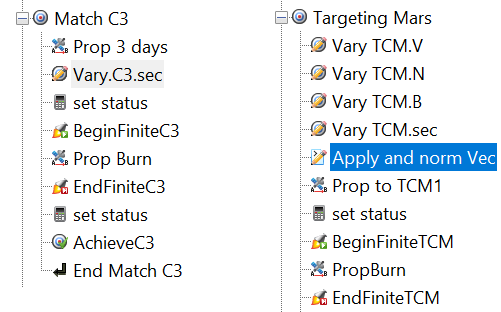
\includegraphics[width=0.7\linewidth]{img/gmat_finite.png}
  \caption{Finite Burn Implementation: standard (left) and multi vectorial (right)}
  \label{fig:gmat-finite}
\end{figure}

\subsubsection{Electric Circularization Logic}
\
\\
When performing electric maneuvers, the maneuver usually spreads over many orbital rounds. This requires a new GMAT structure and was solved with a "while loop" that is repeating a sequence until in the case of maneuver "Circularize" the eccentricity of the orbit is low enough to continue the mission.
Inside this circularization sequence, two thrust arcs are defined by true anomaly (TA).
One centered around the Apoapsis to increase velocity and therefore increase the Periapsis. And the second one centered around its Periapsis to decrease velocity and therefore decrease the Apoapsis. Since the time spend around its Periapsis is much shorter for an highly eccentric orbit, the TA range for the periapsis thrust arc from 270° to 90° (180° span) is substantially higher compared to the apoapsis thrust arc of 179° to 181° (2° span).
In order to keep track of the maneuvers burn time, the elapsed time for each thrust arc is measured and added to a sum by a ScriptEvent. Since one repetition of this static loop section is decreasing the eccentricity in steps, a second "while loop" with identical structure but smaller TA ranges is appended afterwards to reduce the eccentricity in even smaller steps that ultimately achieve an eccentricity of smaller than 0.001. In Figure \ref{fig:gmat-loop} these two "while loops" are shown in its GMAT structure.

\begin{figure}[H]
  \centering
  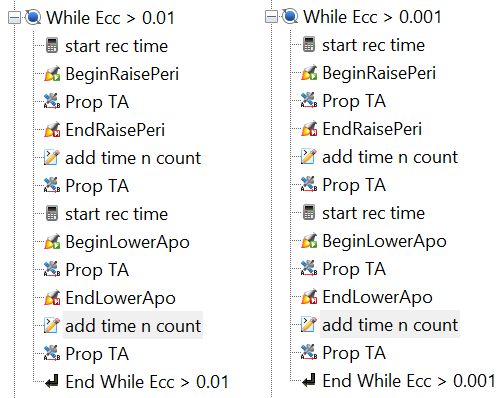
\includegraphics[width=0.7\linewidth]{img/gmat_loop.png}
  \caption{Electric Arcing Structure through While Loops}
  \label{fig:gmat-loop}
\end{figure}

\subsection{GMAT Evaluation}

To process the created values from the GMAT script in a more convenient way, small python scripts are used.
The \href{https://github.com/Sven-J-Steinert/MomenTUM/blob/main/GMAT/plot.py}{\colorbox{codegray}{plot.py}} script is converting the .txt data into a dataframe which is then plotted.
The created plot can be seen in Figure \ref{fig:py-plot}.
The altitude to Mars is plotted in the upper part at the time of the closest encounter during the MOI maneuver. It is of importance that during that finite burn the altitude does not fall into the range of the martian atmosphere. By this knowledge the target altitude of the TCM maneuver is increased until around 250 km altitude are achieved at the closest approach. The targeted altitude of the TCM maneuver and the actual achieved altitude differ due to a back-propagation to apply the MOI burn more centered, which therefore lowers the altitude of the closest approach during the burn.

\begin{figure}[H]
  \centering
  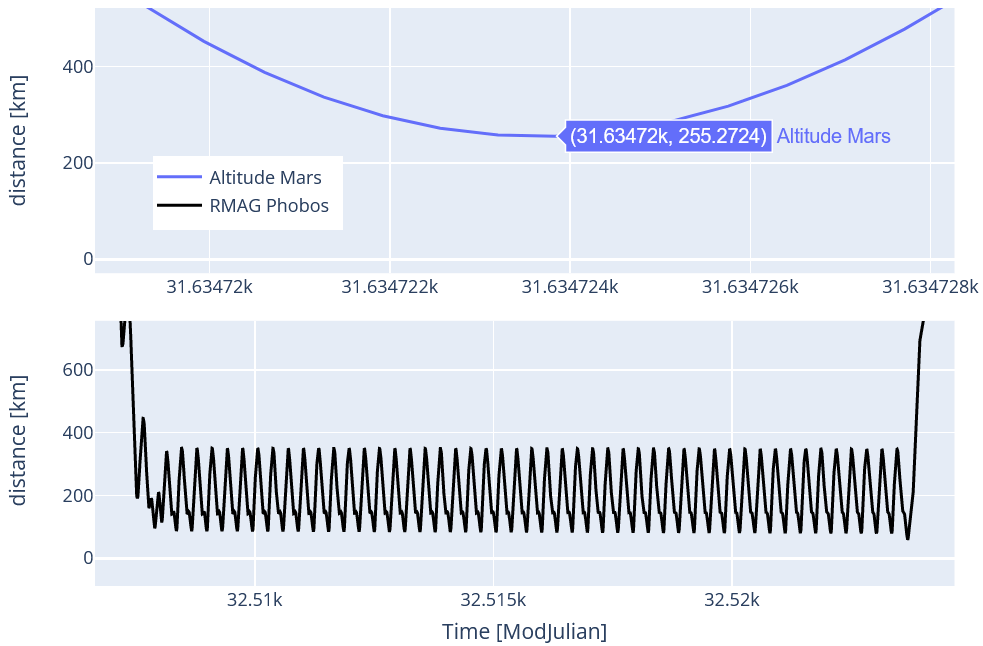
\includegraphics[width=\linewidth]{img/py_plot.png}
  \caption{Plotting of critical values of GMAT by plot.py}
  \label{fig:py-plot}
\end{figure}

The second part of the plot, the lower half, shows the radial magnitude (RMAG) to the center of Phobos.
The sliced time aligns with the arrival at Phobos and the propagation in its quasi stationary orbit.
Even though the matching is automated in the GMAT script to align the phase shift with the waiting time, the GMAT script requires a fixed semi major axis that should be achieved. As experimentation has shown, the semi-major axis of Phobos and therefore its orbital period vary over time. To now set the semi major axis correctly, the plotted evolution of distance is giving information of misalignment in orbital period and therefore semi major axis. This information was fed back until the evolution of RMAG showed no visible drift. The resulting quasi stationary orbit and its stability at the time of arrival over 15 days can be seen in Figure \ref{fig:gmat-orbit}.

\begin{figure}[H]
  \centering
  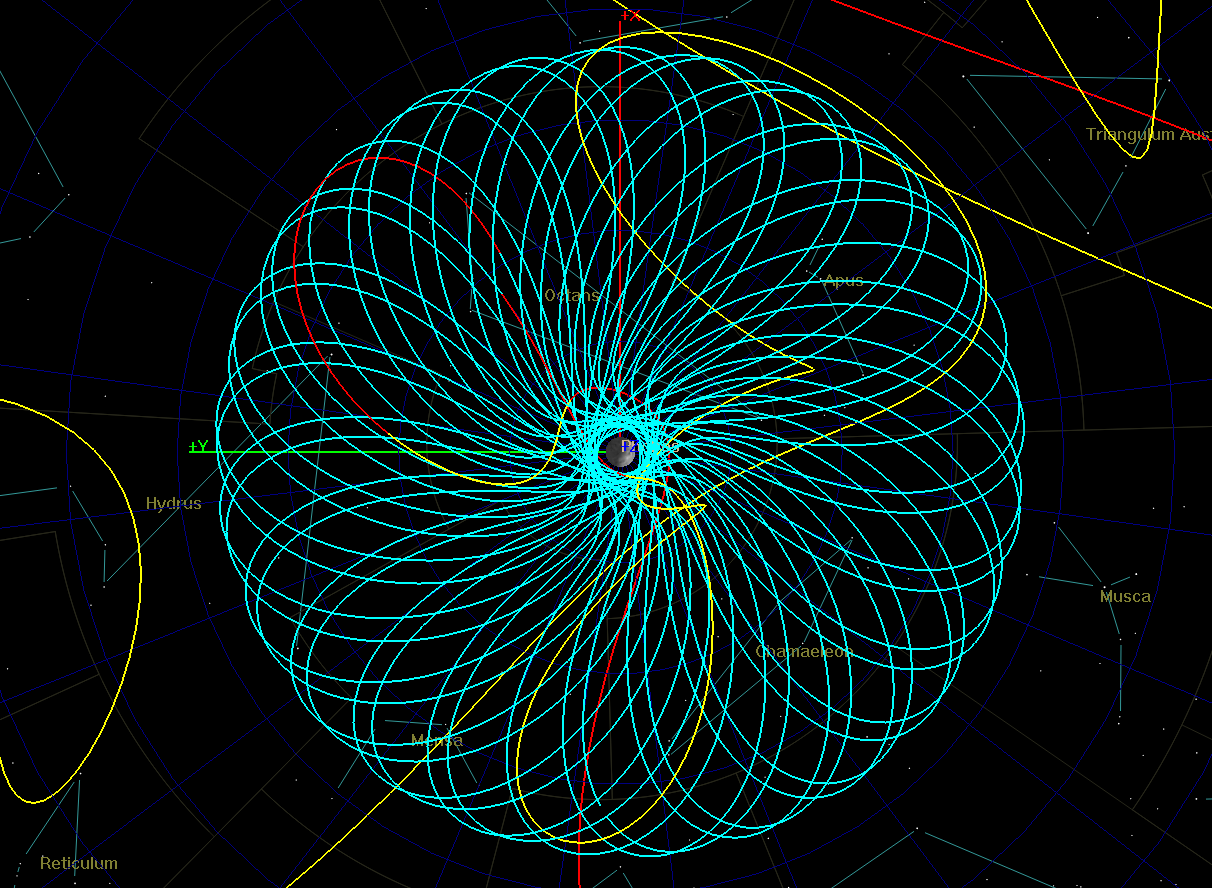
\includegraphics[width=\linewidth]{img/gmat_orbit.png}
  \caption{Resulting Quasi Satellite Orbit around Phobos}
  \label{fig:gmat-orbit}
\end{figure}

\subsection{Selection and Verification}
The selection of the thrusters and the surrounding system was strongly interconnected to the process of developing the trajectory.
By "trying out" several options, the GMAT simulation showed if that system was able to carry out the planned trajectory or not.
Either the trajectory was altered to fit the new needs, if that was possible, or the trajectory did set requirements in return that then decided our selection.
One example being the MOI maneuver that restricted the chemical thruster, where ones with very low thrust have not being able to perform the catch in time before leaving the martian sphere of influence again.
For the electric thruster very low thrust systems created problems in computation time of the GMAT script, which was improved by creating a custom "NearMarsBigStep" propagator that utilizes bigger steps. However, this has its limits as well and even there was no requirement given in flight time, the increasing intensive computation essentially created a limit there too.
The GMAT script also served as validation for matching fuel margins by its leftover fuel in the end of the mission.
The initial fuel mass was adapted and re-runned in GMAT until the defined margin levels did align closely with the leftover fuel at the end.

\subsection{Siemens NX Modelling}

To gain a better understanding of relative sizing from the selected parts and the structure assembly overall, a 3D model of the spacecraft was created. Hereby individual parts as the Xenon, Helium, MMH and MMO tanks as well as main thruster, RCS thruster, electric thruster and solar arrays have been modeled. As an example the electric thruster can be seen in Figure \ref{fig:nx-pps} below.

\begin{figure}[H]
  \centering
  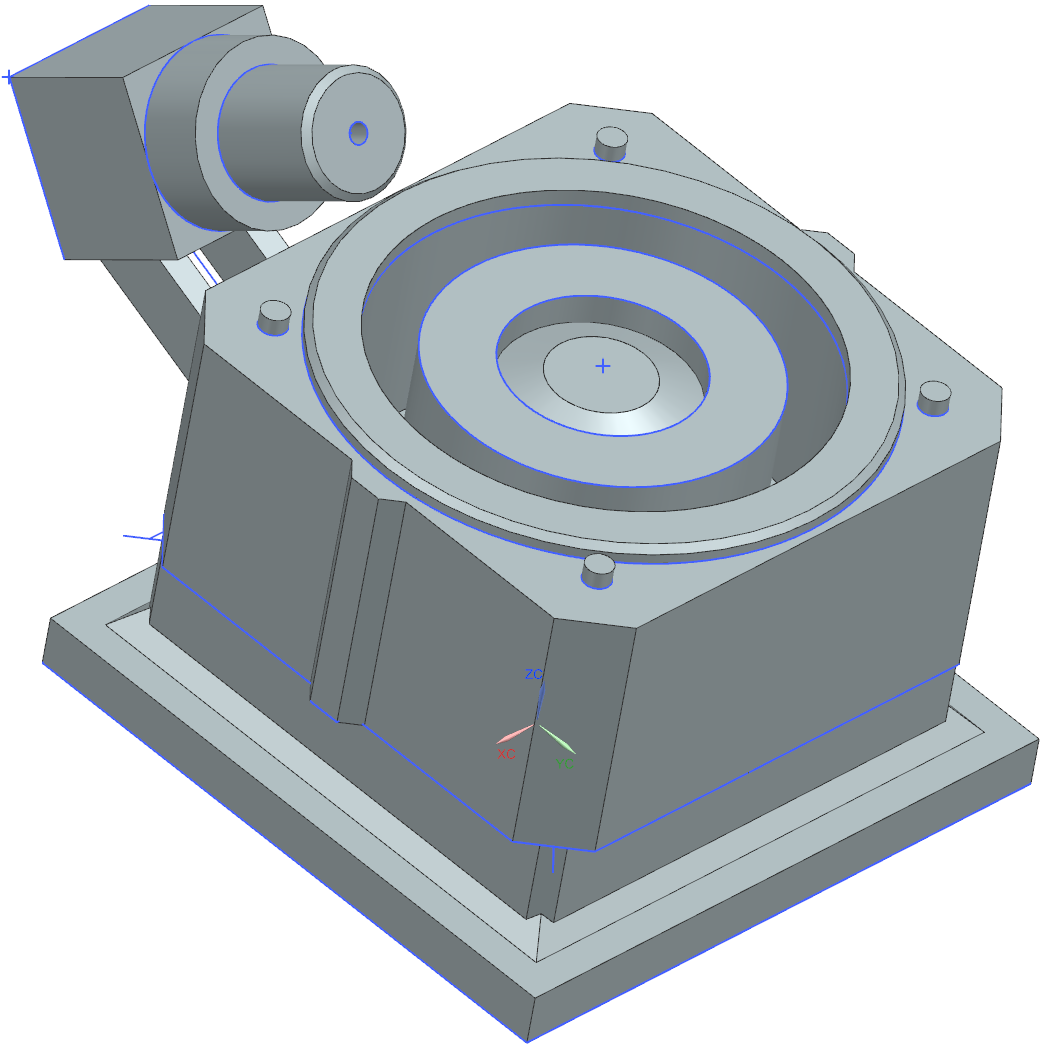
\includegraphics[width=0.7\linewidth]{img/nx_pps.png}
  \caption{3D model of the Safran PPS 1350 Hall Effect Thruster}
  \label{fig:nx-pps}
\end{figure}

The three-dimensional alignment of parts and spacial piping gave important insights for the arrangement analysis and the pipe mass estimation. The resulting arrangement can be found in \href{https://github.com/Sven-J-Steinert/MomenTUM/blob/main/NX/Assembly_MomenTUM.prt}{\colorbox{codegray}{Assembly\_MomenTUM.prt}}.
\\

\subsection{Documentation}
To provide better access to all the files that have been created, a \href{https://github.com/Sven-J-Steinert/MomenTUM}{\colorbox{codegray}{GitHub Repository}} was created.
All grey boxes inside this document are leading to their corresponding file in the repository.
The documentation was done in LaTeX which source code is also given in the \href{https://github.com/Sven-J-Steinert/MomenTUM/tree/main/doc}{\colorbox{codegray}{doc}} folder.